\documentclass[a4paper]{article}

%% Language and font encodings
\usepackage[english]{babel}
\usepackage[utf8x]{inputenc}
\usepackage[T1]{fontenc}
\usepackage{graphicx}
\usepackage{float}
\usepackage{amsmath}

%% Sets page size and margins
%\usepackage[letter,top=3cm,bottom=2cm,left=3cm,right=3cm,marginparwidth=1.75cm]{geometry}

%% Useful packages
\usepackage{amsmath}
\usepackage{graphicx}
\usepackage[colorinlistoftodos]{todonotes}
\usepackage[colorlinks=true, allcolors=blue]{hyperref}

\title{CS534 - Implementation Assignment 4}
\date{\today}
\author{Peter Rindal, Hung Viet Le, and Trung Viet Vu}

\begin{document}
\maketitle



%\section{Group Information}
\begin{table}[H]
\begin{center}
  \begin{tabular}{ | c | c | c | }
    \hline
    Member Name & OSU ID & Contribution \\ \hline
    Peter Rindal & 931731553 & 33.33\% \\ \hline
    Hung Viet Le & 932259606 & 33.33\% \\ \hline
    Trung Viet Vu & 932986775 & 33.33\% \\
    \hline
  \end{tabular}
\end{center}
\end{table}

In this assignment, we implement two dimension reduction methods, namely Principle Component Analysis (PCA) and Linear Discriminant Analysis (LDA). We also implement K-Means as a clustering algorithm for the provided data set, which is a 2059x477 processed-matrix measured from walking up and down stairs activity.


\section{Apply K-Means to the original data}
For the first part, we apply the general K-Means algorithm to the original data. The maximum number of iteration for K-Means is set to 50, and we randomly restart this algorithm 10 times. The solution with the best Sum Squared Error (SSE) is 355, with class 0 and 1's purities are 75.55\% and 89.00\%, respectively.
The result is quite good, reaching an average of more than 80\% accuracy. It can also be seen that the resulting assignment gets better performance on walking down data (class 1).


\section{Compute the principle components of the data}
The first 10 principle components variances are given in Figure 1. In order to retain at least 80\% and 90\% of the total variance, the smallest dimension we can reduce to is 27 and 57, respectively. Recall that there are 477 features in total. This shows that while roughly 10\% of them contain useful information, the remaining 90\% are actually redundant and irrelevant features.

\begin{figure}[H]
\begin{center}
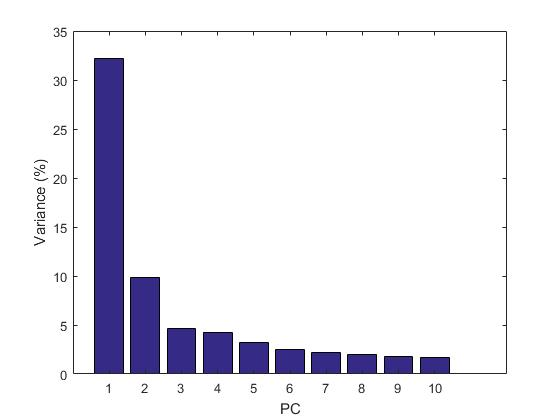
\includegraphics[width=5in]{PCs.jpg}
\caption{First 10 principle components variances}
\end{center}
\end{figure}


\section{Apply PCA to reduce the data dimension}
The resulting reduced data when applying K-Means is reported in Table 1. As can be seen from the table, class purity is slightly smaller than the result reported in Section 1. This can be explained by the fact that a lot of information has been removed from the original data. It is noteworthy that K-Means algorithm runs much faster in the later case, yet achieving a relatively good result compared to the former one.

Additionally, the figure suggests that as we increase the number of principle components from 1 to 2, the accuracy increase by nearly 3\%. However, this trend is not observed when the number of PCs increases from 2 to 3. One explanation is that the result is already as good as the result for original data, and if we wish to see some significant improvement, more PCs need to be added, for example adding up to 27 and 57 PCs.


\begin{table}
\centering
\begin{tabular}{ | c | c | c | c | }
\hline
Data & Best SSE & Class 0 Purity & Class 1 Purity \\ \hline
Original & 355 & 75.55 & 89.00 \\ \hline    
PCA-1 & 415 & 72.61 & 86.48 \\ \hline
PCA-2 & 360 & 75.55 & 88.90 \\ \hline
PCA-3 & 360 & 75.55 & 88.90 \\ \hline
LDA & 355 & 75.55 & 89.00 \\ \hline
\end{tabular}
\caption{Best SSE and class purities for different settings}
\end{table}


\section{Apply LDA to reduce the data dimension}
The result for Linear Discriminant Analysis is described in Table 1. It is the same as the result when we apply K-Means to the original data, which is very good in terms of performance. And clearly, this result is better than ones obtained in  PCA-1,2,3.



\section{Discuss the suitability of PCA and LDA}
For this particular dataset, we choose LDA as the winner. Basically, LDA as a supervised method tries to identify attributes that account for the most variance between classes, while PCA (unsupervised) tries to retain as much data variance as possible. In this assignment, since LDA uses known class labels - which is given in the dataset, it performs better than PCA.



\end{document}
















